\documentclass[a4paper,12pt]{article}

\usepackage[utf8]{inputenc}
\usepackage[polish]{babel}
\usepackage{polski}
\usepackage{a4wide}

\usepackage[colorlinks=true,linkcolor=blue]{hyperref}

\usepackage[pdftex]{graphicx}



\usepackage{microtype}

\hypersetup{
unicode = true,
pdfauthor = {Daniel Kłobuszewski, Jakub Kotur, Jan Stępień},
pdftitle = {Cumulonimbus -- Dokumentacja końcowa},
pdfsubject = {RSO 11L}
}

\def\cb{Cumulonimbus}
\def\todo{\textbf{TODO}: }

\title{\cb{} \\ Dokumentacja końcowa}
\author{Daniel Kłobuszewski \and Jakub Kotur \and Jan Stępień}

\begin{document}

\maketitle
\csname @starttoc\endcsname{toc}

\section{Architektura}
\documentclass[a4paper,12pt]{article}

\usepackage[utf8]{inputenc}
\usepackage[polish]{babel}
\usepackage{polski}
\usepackage{a4wide}

\usepackage[colorlinks=true,linkcolor=blue]{hyperref}

\usepackage[pdftex]{graphicx}



\hypersetup{
	unicode = true,
	pdfauthor = {Daniel Kłobuszewski, Jan Stępień},
}

\title{Cumulonimbus -- Architektura Systemu}
\author{Daniel Kłobuszewski \and Jan Stępień}

\def\cb{Cumulonimbus}
\def\todo{\textbf{TODO}: }

\begin{document}

\maketitle

\section{Swift}

Do realizacji projektu \cb{} wykorzystany został projekt OpenStack Storage, znany
również jako Swift. Wyczerpujący opis tego narzędzia znajduje się w~jednym
z~dokumentów dostarczonych na początku semestru \cite{qba-swift}, stąd
w~niniejszym dokumencie nie będziemy zajmować się szczegółami jego działania.
Ograniczamy się jedynie do przypomnienia, że Swift to rozproszony system
bazodanowy pozwalający na redundancyjne przechowywanie plików w~kontenerach
o~płaskiej strukturze.

\subsection{Konfiguracja}

Projekt \cb{} wymaga do swojego działania dostępu do działającego klastra Swift
o~dowolnej architekturze. Prace deweloperskie były prowadzone na minimalnej
instancji uruchomionej na pojedynczej maszynie wirtualnej. Testy w~laboratorium
wykonywano na bardziej rozbudowanej instalacji z~serwerami danych rozproszonymi
na kilku maszynach fizycznych. \todo oby to była prawda.

Sposób konfiguracji minimalnej instancji Swift potrzebnej do działania projektu
\cb{} -- Swift All In One -- został przedstawiony w~dokumentacji Swift
\cite{swift_doc}. Rozwiązanie to powoduje uruchomienie serwera autoryzującego,
serwera pośredniczącego oraz czterech serwerów danych na jednej maszynie
fizycznej. Alternatywne rozwiązania umożliwiają uruchomienie każdego
z~powyższych serwerów na różnych maszynach fizycznych, co nadaje całemu
rozwiązaniu cechy systemów \textit{fault-tolerant}.

\subsection{Zalety}

Projekt \cb{} jest niezależny od sposobu konfiguracji klastra Swift. Może być to
zarówno minimalna instancja uruchomiona na pojedynczej maszynie fizycznej, jak
i~rozproszony system wielu instancji. Dzięki poziomowi przezroczystości
zapewnianej przez Swift sposób jego instalacji nie ma znaczenia dla projektu
\cb{}. Przezroczystość ta pozwala projektowi \cb{} na udostępnienie
użytkownikowi systemu plików o~szeregu zalet.

Po pierwsze, Swift gwarantuje redundancyjne mechanizmy przechowywania danych
oraz \textit{fault-tolerance}. W~wypadku uszkodzenia pewnej części węzłów
klastra przechowujących dane system plików \cb{} może nadal działać poprawnie,
pod warunkiem, że awaria nie zaburzy działania samego systemu Swift. Jeżeli
zapewnieni autorów Swift są poprawne, użytkownik nie powinien odczuć żadnych
konsekwencji tego typu zdarzeń.

Drugą zaletą jest możliwość złączenia w~ramach klastra Swift dowolnie dużej
przestrzeni dyskowej. W~efekcie \cb{} pozwala na przechowywanie wielkiej ilości
danych, które zostaną automatycznie rozlokowane pomiędzy dyskami wchodzącymi
w~skład maszyn tworzących wykorzystywany przez \cb{} klaster.

Trzecią zaletą jest wysoki poziom abstrakcji interfejsu Swift, który udostępnia
jedynie podstawowe funkcje odpowiadające za mechanizmy przechowywania
i~odzyskiwania danych. Mechanizmy redundancyjnego rozmieszczania danych
w~klastrze, wydajnego wyszukiwania obiektów potrzebnych do zrealizowania żądania
użytkownika czy też zapewnienie spójności pomiędzy serwerami danych jest
dokonywane automatycznie. Jako autorzy systemu plików nie musimy też rozwiązywać
skomplikowanego zagadnienia jakim jest fragmentacja partycji.

\section{FUSE}

\begin{figure}
	\centering
	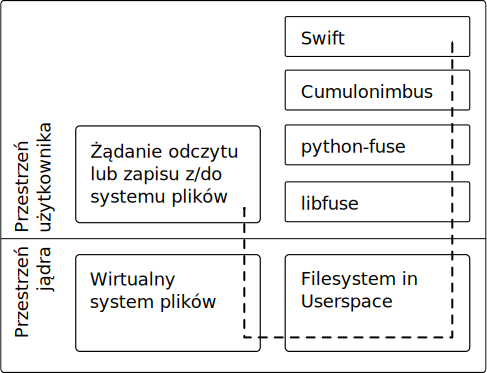
\includegraphics[width=0.6\textwidth]{fuse.pdf}
	\caption{Architektura systemu}
	\label{fig:fuse}
\end{figure}

W~systemie operacyjnym Linux systemy plików implementowane są i~działają w
przestrzeni adresowej jądra. Istnieje jednak możliwość implementacji takiego
systemu w~przestrzeni użytkownika. Pozwala na to biblioteka FUSE -- Filesystem
in Userspace. Odpowiada ona za przekazywanie niskopoziomowych wywołań systemu
plików do procesu użytkownika.

Dzięki temu możliwa jest implementacja pełnoprawnego systemu plików bez
jakiejkolwiek ingerencji w~kod jądra. Niewątpliwą wygodą tego rozwiązania
jest fakt, że żaden błąd w~takiej implementacji nie może zakłócić działania
jądra systemu -- inaczej niż w~tradycyjnych systemach plików.

Kolejną zaletą tej biblioteki jest obecność bindingów do różnych języków
programowania, w~tym do Pythona, na którego użycie się zdecydowaliśmy.

\section{Implementacja systemu plików}

\begin{figure}
    \centering
    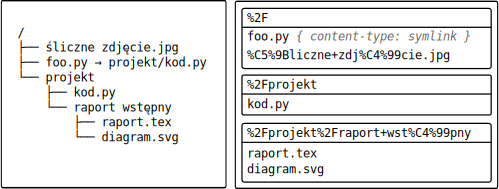
\includegraphics[width=0.7\textwidth]{drzewo.pdf}
    \caption{Przykładowe drzewo katalogów}
	\label{fig:drzewo}
\end{figure}

Projekt \cb{} implementuje prosty system plików. Wspiera kluczowe dla normalnej
pracy operacje, takie jak tworzenie, odczyt, modyfikacja i~usuwanie katalogów
i~plików. Wspierane są również dowiązania symboliczne. Poza zakresem prac
znalazły się wielokrotne dowiązania twarde -- każdy plik ma tylko jeden hard
link.

Każdy katalog jest reprezentowany jako osobny kontener o~unikalnej nazwie będącą
ścieżką danego katalogu zakodowaną przy pomocy kodowania \textit{URL-encoding}.
Wewnątrz kontenera przechowywane są znajdujące się w~odpowiadającym mu katalogu
pliki i~dowiązania symboliczne. Każdy plik i~dowiązanie przechowywany jest jako
obiekt w~rozumieniu pakietu Swift. Nazwy obiektów to ostatnia część nazwy
odpowiedniego pliku lub dowiązania, również zakodowana przy pomocy
\textit{URL-encoding}. Do realizacji kodowania i~dekodowania
\textit{URL-encoding} wykorzystany został moduł \texttt{urlib} wchodzący w skład
standardowej biblioteki Pythona 2.6 i~nowszych.

Zawartość plików przechowywana jest jako zawartość reprezentujących je obiektów.
Dowiązania symboliczne są wyróżnione wartością przypisanego każdemu Swiftowemu
obiektowi pola \texttt{content-type} -- w~ich wypadku ma ono wartość
\texttt{symlink}. Zwykłe pliki mają w~tym miejscu standardowy typ zawartości,
\texttt{application/octet-stream}. Ponadto treść obiektu reprezentującego
dowiązanie symboliczne to ścieżka do wskazywanego przezeń pliku. Informacje
o~czasie ostatniej modyfikacji obiektów przechowywane są w~analogicznym do
\texttt{content-type} polu z~metadanymi \texttt{last-modified}.

Przykładową reprezentację minimalnego systemu plików przedstawiono na rysunku
nr~\ref{fig:drzewo}. Z~lewej strony widoczne jest drzewo katalogów, z~prawej
natomiast trzy kontenery Swift przechowujące reprezentację drzewa. Na diagramie
pominięto pole \texttt{content-type} zwykłych plików.

\paragraph{}
Opisany sposób implementacji posiada niestety pewne wady. Wynikają one z
przyjętej przez nas architektury oraz założeń Swifta. Przede wszystkim \cb{}
kiepsko radzi sobie z~dużymi plikami -- API Swifta nie pozwala na podmienianie
części pliku, więc każda zmiana w~pliku niesie ze sobą konieczność przesłania
całej jego zawartości.

Nie ma także możliwości zmiany nazwy obiektu w~kontenerze, przez co każda zmiana
nazwy pliku sprowadza się do pobrania go w~całości na lokalny komputer, po czym
wysłania z~powrotem z~inną nazwą. To samo dotyczy katalogów.

Ostatni problem, którego nie rozwiązaliśmy ze względu na założenie minimalności
implementacji, to synchronizacja podczas jednoczesnej pracy kilku użytkowników.
W~obecnej postaci \cb{} nadaje się tylko do jednoczesnego korzystania przez
jednego użytkownika.

\section{Instrukcja obsługi}
Użycie naszego projektu różni się od standardowego użycia systemu plików
jedynie sposobem montowania i~demontowania. Cała reszta poleceń powłoki
i~wywołań I/O~jest identyczna.

\subsection{Zależności}

Do instalacji i~poprawnego działania projektu \cb{} niezbędna jest instalacja
następujących aplikacji i~biblioteki, wraz z~ich zależnościami.

\begin{itemize}
	\item{Python 2.6}
	\item{python-fuse 0.2.1}
	\item{swift, wersja z~systemu kontroli wersji, rewizja 257 \todo dlaczego
		ta konkretna}
\end{itemize}

\subsection{Instalacja}

Dalsze sekcje będą zakładały, że została wykonana poprawna instalacja a~główny
skrypt programu znajduje się w~jednym z~katalogów ze~zmiennej środowiskowej
\texttt{PATH}. Poniższe polecenie wykonane w~głównym katalogu ze źródłami
zainstaluje \cb{} w~katalogu \texttt{/usr/local}.

\begin{verbatim}
./setup.py install
\end{verbatim}

Jeżeli \cb{} ma być zainstalowany w~innym miejscu należy wykorzystać opcję
\texttt{--prefix}:

\begin{verbatim}
./setup.py install --prefix /absolute/destination/path
\end{verbatim}

Więcej informacji na temat procedury instalacji i~możliwych opcji można uzyskać
przy pomocy opcji \texttt{--help}.

\begin{verbatim}
./setup.py --help
\end{verbatim}

\subsection{Montowanie}

Aby zamontować system plików używamy polecenia:

\begin{verbatim}
cumulonimbus <mountpoint> <opcje>
\end{verbatim}

Opcje wbrew nazwie nie są opcjonalne. Pierwsza z~nich to authurl -- adres URL
serwera autoryzacji. Kolejne dwie to user oraz key -- czyli użytkownik oraz
jego hasło na tym serwerze.

Opcje podajemy po fladze -o:

\begin{verbatim}
cumulonimbus dir -o authurl=http://127.0.0.1:8080/auth/v1.0 \
    -o user=test:tester -o key=testing
\end{verbatim}

Warto zwrócić uwagę na charakterystyczny dwukropek w~nazwie użytkownika.
Oddziela on pierwszy człon nazwy -- konto -- od drugiego -- faktycznej nazwy.
Na jednym koncie może znajdować się wielu użytkowników, każdy z~innymi
uprawnieniami.

\subsection{Demontowanie}

Demontowanie jest na szczęście znacznie prostsze:

\begin{verbatim}
fusermount -u <mountpoint>
\end{verbatim}

\section{Możliwości rozwoju}

\subsection{Synchronizacja użytkowników}
Aby \cb{} mógł stać się rozwiązaniem, które sprawdzi się w~praktyce, konieczna
byłaby implementacja mechanizmu synchronizacji, który zapobiegłby uszkodzeniu
plików, na przykład poprzez uniemożliwienie jednoczesnej edycji przez różnych
użytkowników. Mechanizm taki musiałby radzić sobie z~sytuacjami, w~których
zerwaniu ulega połączenie z~użytkownikiem.

\bibliographystyle{../plplainurl}
\bibliography{../bibliografia}

\end{document}


\section{Instrukcja obsługi}
Użycie naszego projektu różni się od standardowego użycia systemu plików
jedynie sposobem montowania i~demontowania. Cała reszta poleceń powłoki
i~wywołań I/O~jest identyczna.

\subsection{Zależności}\label{sec:zaleznosci}

Do instalacji i~poprawnego działania projektu \cb{} niezbędna jest instalacja
następujących aplikacji i~biblioteki, wraz z~ich zależnościami.

\begin{itemize}
	\item{Python 2.6}
	\item{python-fuse 0.2.1}
	\item{swift, nowszy lub równy wersji 1.3}
\end{itemize}

Biblioteka kliencka Swifta jest jeszcze mocno niedopracowana. Do tego stopnia,
że podstawowe wywołania API rzucają wyjątkami wskazującymi na literówki
w~kodzie Swift. Od wersji 1.3 wzwyż, tylko jeden z~tego typu wyjątków był
spowodowany błędami w~naszym kodzie. Aby uruchomić projekt, należy usunąć 3
linie odpowiedzialne za logowanie w~kodzie Swifta -- to one powodują błędy
i~wyjątki. Warto w~tym miejscu zaznaczyć, że na początku semestru zgłosiliśmy
ten błąd developerom Swifta i~do tej pory nie uzyskaliśmy
odpowiedzi~\cite{launchpad-bug}.

\subsection{Instalacja}

Dalsze sekcje będą zakładały, że została wykonana poprawna instalacja a~główny
skrypt programu znajduje się w~jednym z~katalogów ze~zmiennej środowiskowej
\texttt{PATH}. Poniższe polecenie wykonane w~głównym katalogu ze źródłami
zainstaluje \cb{} w~katalogu \texttt{/usr/local}.

\begin{verbatim}
./setup.py install
\end{verbatim}

Jeżeli \cb{} ma być zainstalowany w~innym miejscu należy wykorzystać opcję
\texttt{--prefix}:

\begin{verbatim}
./setup.py install --prefix /absolute/destination/path
\end{verbatim}

Więcej informacji na temat procedury instalacji i~możliwych opcji można uzyskać
przy pomocy opcji \texttt{--help}.

\begin{verbatim}
./setup.py --help
\end{verbatim}

\subsection{Montowanie}

Aby zamontować system plików używamy polecenia:

\begin{verbatim}
cumulonimbus <mountpoint> <opcje>
\end{verbatim}

Opcje wbrew nazwie nie są opcjonalne. Pierwsza z~nich to authurl -- adres URL
serwera autoryzacji. Kolejne dwie to user oraz key -- czyli użytkownik oraz
jego hasło na tym serwerze.

Opcje podajemy po fladze -o:

\begin{verbatim}
cumulonimbus dir -o authurl=http://127.0.0.1:8080/auth/v1.0 \
    -o user=test:tester -o key=testing
\end{verbatim}

Warto zwrócić uwagę na charakterystyczny dwukropek w~nazwie użytkownika.
Oddziela on pierwszy człon nazwy -- konto -- od drugiego -- faktycznej nazwy.
Na jednym koncie może znajdować się wielu użytkowników, każdy z~innymi
uprawnieniami.

\subsection{Demontowanie}

Demontowanie jest na szczęście znacznie prostsze:

\begin{verbatim}
fusermount -u <mountpoint>
\end{verbatim}


\section{Problemy z autoryzacją}
\documentclass[a4paper,12pt]{article}

\usepackage[utf8]{inputenc}
\usepackage[polish]{babel}
\usepackage{polski}
\usepackage{a4wide}

\usepackage[colorlinks=true,linkcolor=blue]{hyperref}

\usepackage[pdftex]{graphicx}



\usepackage{microtype}

\hypersetup{
	unicode = true,
	pdfauthor = {Jakub Kotur},
}

\title{Cumulonimbus\\\large{wnioski z projektowania autoryzacji}}
\author{Jakub Kotur}

\begin{document}
	\maketitle

	\section{Stan projektu}\label{sec:stan projektu}

	Projekt w momencie kiedy pisany jest ten dokument jest w pełni funkcjonalnym systemem plików. Można wykonywać takie operacje jak tworzenie i usuwanie katalogów i plików, zapisywanie danych do pliku, oraz tworzenie linków symbolicznych. Dokładny opis tego co zostało zrobione i jak działa, zawarty jest w dokumentacji projektu. Pierwotne założenia projektu zakładały też pełny system ACL dla plików i katalogów. Po kilku próbach rozwiązania tego problemu, doszliśmy do wniosku, że nie ma możliwości prostego sposobu na implementacje tej funkcjonalności. Ten dokument opisze nasze prace nad tym zagadnieniem i wnioski jakie z nich wyciągnęliśmy.
	
	\section{Wsparcie ACL przez Swift}\label{sec:wsparcie acl przez swift}

	Pierwsze podejście do zagadnienia systemu autoryzacji w Swifcie było bardzo pozytywne. Według dokumentacji Swift wspiera pełny system ACL, więc sądziliśmy że nie będzie najmniejszego problemu z użyciem go w naszym projekcie. Aby użyć tego systemu, trzeba używać serwera autoryzacji swauth, ale tutaj też czekała nas miła niespodzianka, ponieważ w wersji 1.3 Swifta, domyślnym systemem autoryzacji jest swauth. Szybko udało się więc skonfigurować wszystko, tak aby utworzyć konta użytkowników i zacząć testy.

	W dokumentacji jest napisane, że aby ustawić uprawnienia użytkownikowi do kontenera, należy wpisać w dodatkowych nagłówkach \texttt{'x-container-read'} i \texttt{'x-container-write'} użytkownika. Po kilku próbach okazało się, że poprawną nazwą użytkownika jest \texttt{<nazwa konta>:<login użytkownika>}. Po wpisaniu przez administratora poprawnych wartości w~powyższe pola użytkownik uzyskuje dostęp do kontenera.

	Niestety na tym skończyły się sukcesy z używaniem systemu ACL. Okazało się że użytkownik nie jest w stanie przeczytać zawartości konta, do którego się zalogował. Jedyne co jest napisane w dokumentacji na temat autoryzacji, to wymienione powyżej nagłówki. Na próżno szukaliśmy kolejnych informacji na temat autoryzacji w Swifcie w Internecie. Dopiero zajrzenie w~źródła projektu dało odpowiedź na pytanie, co dalej. Okazało się że jedynym miejscem gdzie Swift komunikuje się z swauth i wymienia informacje o ACLkach są właśnie kontenery. Działa to w ten sposób, że jeżeli użytkownik ma uprawnienia do pisania do kontenera, to może tworzyć i nadpisywać wszystkie obiekty w nim zawarte, analogicznie jest z czytaniem. Oznacza to też że nie ma żadnej możliwości operacji na kontenerach przez użytkownika. Nie może on ani listować, ani tworzyć kontenerów.

	Pomyśleliśmy więc że musimy sobie radzić z tym co mamy i rozpatrzyliśmy dwie zupełnie odmienne architektury.
	
	\section{Projekty architektury}\label{sec:projekty architektury}

	\subsection{Projekt bezpośredni}\label{sub:projekt bezposredni}

	Pierwszym projektem kiedy jeszcze nie wiedzieliśmy jak wygląda system autoryzacji w Swifcie, był projekt bezpośredni, gdzie folderowi odpowiada kontener, a plikowi obiekt. Jest to prosty i intuicyjny projekt, w którym synchronizacja i tranzakcyjność zapewnione są przez Swifta. Dokładny opis tego rozwiązania znajduje się w dokumentacji, ponieważ ostatecznie zdecydowaliśmy się na tę wersję architektury. W tym miejscu należy zauważyć, że pierwotnie pomysł ten przepadł ze względu na kompletny brak możliwości implementacji uprawnień przy pomocy Swifta. Ponieważ wszystkie obiekty mają takie same uprawnienia w danym kontenerze, a kontenerów w koncie nie da się w ogóle listować, taki projekt nie mógł mieć systemu uprawnień zapewnionego przez Swifta.
	
	\subsection{Projekt kontenerów}\label{sub:projekt kontenerow}

	Drugim projektem, który miał duże szanse powodzenia, był pomysł tworzenia dla każdego obiektu (czyli katalogu, pliku, dowiązania) kontenera opisującego ten obiekt. Pomysł jest już trochę trudniejszy w implementacji, ponieważ należy dbać o synchronizację i poprawność struktury kontenerów. Może też cierpieć na utratę danych, ponieważ jeżeli utracimy opis katalogu, tracimy też dostęp do wszystkich podkatalogów. W zamian zyskujemy o wiele szybsze operacje przenoszenia i zapisu danych. Z punktu widzenia systemu autoryzacji ten projekt też był bardzo obiecujący. Ponieważ w Swifcie tyko kontenery mają swoje uprawnienia, to bylibyśmy w stanie opisać uprawnienia systemu plików, uprawnieniami Swifta. Istnieje jednak jeden istotny problem, który przekreślił to rozwiązanie zupełnie. Okazało się, że zwykły użytkownik w systemie Swift nie jest w stanie utworzyć kontenera. Ten fakt spowodował, że również to rozwiązanie zostało porzucone.

	\subsection{Podsumowanie}\label{sub:podsumowanie}
	
	Oba rozwiązania przedstawione w tym rozdziale są poprawne i dobrze spełniają swoje zadanie. W obu jednak nie byliśmy w stanie zapewnić autoryzacji przy pomocy narzędzi udostępnionych przez Swifta. Podejrzewamy że spowodowane to jest młodym stadium rozwoju projektu Swift. Ponieważ Swift jest bardzo aktywnie rozwijany, najprawdopodobniej niedługo pojawią się narzędzia pozwalające na szersze nadawanie uprawnień, tak że będzie można z poziomu użytkownika tworzyć katalogi. Najlepszym rozwiązaniem jest więc poczekać i zobaczyć które rozwiązanie szybciej stanie się możliwe.
	
	\section{Możliwe rozwiązania}\label{sec:mozliwe rozwiazania}

	Poniżej przedstawione zostaną rozwiązania które są możliwe do zaimplementowania ze Swiftem w aktualnej wersji, jednak z różnych powodów nie widzieliśmy sensu ich implementacji. Z powodu ograniczeń w Swifcie, są one kombinowane, także zdecydowanie lepszym rozwiązaniem jest poczekać.

	\subsection{Lokalna autoryzacja}\label{sub:lokalna autoryzacja}

	Aby zapewnić wrażenie autoryzacji i systemu ACL, można stworzyć system autoryzacji lokalnie, tak aby aplikacja sama weryfikowała uprawnienia. To rozwiązanie ma jednak jedną zdecydowaną wadę: zabezpieczenie jest zupełnie fikcyjne. Pomijając ataki typu crackerskiego, jak podmienianie kodu aplikacji, każdy użytkownik znając swoje hasło i swój login, mógłby się po prostu zalogować do Swifta korzystając z jego API i przeczytać pliki mu niedostępne. Szczególnie złośliwy włamywać mógłby też podmienić pliki używane przez nas do autoryzacji, tak aby inni użytkownicy nie mieli do nich dostępu. Takie rozwiązanie, choć możliwe, nie zapewnia żadnego stopnia bezpieczeństwa, co spowodowało, że nie zdecydowaliśmy się na jego implementację.

	\subsection{Rozszerzenie projektu Swift}\label{sub:rozszerzenie projektu swift}

	Ten sam kod, który jest potrzebny do lokalnej autoryzacji, wykonywany zdalnie na serwerze ma już sens. Można zatem uruchomić serwer pośredniczący zajmujący się wyłącznie autoryzacją, albo po prostu rozszerzyć o~tę funkcjonalność projekt Swift. Wystarczyło by zapewne dodać obsługę pól nagłówków \texttt{'x-account-*'} oraz \texttt{'x-object-*'}, analogiczną jak w przypadku \texttt{'x-container-*'}. To rozwiązanie, jakkolwiek dobre, wykracza poza zakres projektu zdalnego systemu plików.
	
	\subsection{Wykorzystanie projektu Nova}\label{sub:wykorzystanie projektu nova}

	\textbf{TODO} asdf asdf asdf!
	
	\section{Wnioski}\label{sec:wnioski}

	Reasumując, stworzyliśmy dwa projekty zdalnego systemu plików, z których każdy ma swoje wady i zalety. Obu jednak nie jesteśmy w stanie stworzyć przy aktualnym stanie projektu Swift. Mimo że Swift wspiera system ACL, jest on zbyt ubogi, aby stworzyć system plików z autoryzacją po stronie serwera. Użytkownik ma albo zbyt małe, albo zbyt duże uprawnienia, do poszczególnych obiektów Swifta. Wpadliśmy też na kilka pomysłów jak zaimplementować system autoryzacji korzystając z aktualnej wersji Swifta, jednak żaden z nich nie był dość zadowalający. Dobre rozwiązanie są zbyt trudne, a te dość proste, są z gruntu błędne. Najlepszym więc rozwiązaniem według nas jest poczekać na rozwój projektu Swift i w zależności od tego jak się rozwinie, zaimplementować jedno z dobrych rozwiązań.

\end{document}



\section{Wnioski końcowe}
\subsection{Swift}

Projekt OpenStack Swift jest jeszcze na dość wczesnym etapie rozwoju. W
efekcie czasem można natknąć się na ewidentne błędy autorów [\todo{tu wstawić opis
błędu}]. Z drugiej jednak strony, na korzyść tegoż projektu przemawia proste
API i dość dobra dokumentacja. Te dwie cechy sprawiają, że korzystanie ze
Swifta jest całkiem proste.

Przedstawione przez nas na początku semestru w~dokumencie \cite{jano-anal-atech}
obawy na temat otwartości procesu powstawania projektu Swift nie okazały się
przesadzone. Jak zauważyliśmy w~sekcji \ref{sec:zaleznosci}, niepokoi nas brak
odpowiedzi na zgłoszone przez nas błędy. Mamy nadzieję, że całość będzie
zmieniać się na lepsze, ale zespołom planującym wykorzystanie Swift w~swoich
rozwiązaniach zalecamy wzięcie tej kwestii pod uwagę.

\subsection{python-fuse}

Zdecydowaliśmy się na implementację systemu plików w Pythonie. Biblioteka FUSE
posiada interfejs w języku C, co implikowało konieczność użycia jakichś
bindingów dla Pythona. Wybór padł na python-fuse. Wygoda ich użycia była
niestety mocno ograniczona przez brak dokumentacji. Na szczęście w internecie
można znaleźć kompletną, "pustą", przykładową implementację. Na jej podstawie
udało nam się zorientować, jak mają wyglądać wszystkie potrzebne funkcje.



\bibliographystyle{../plplainurl}
\bibliography{../bibliografia}

\end{document}
